
\newthought{Let's the fun begin!}
We are left to define what derivatives of functions between manifolds are.
And, since we saw that euclidean spaces are manifolds, we better find a definition that coincides with the one you saw in your analysis courses.

\begin{marginfigure}[7em]
  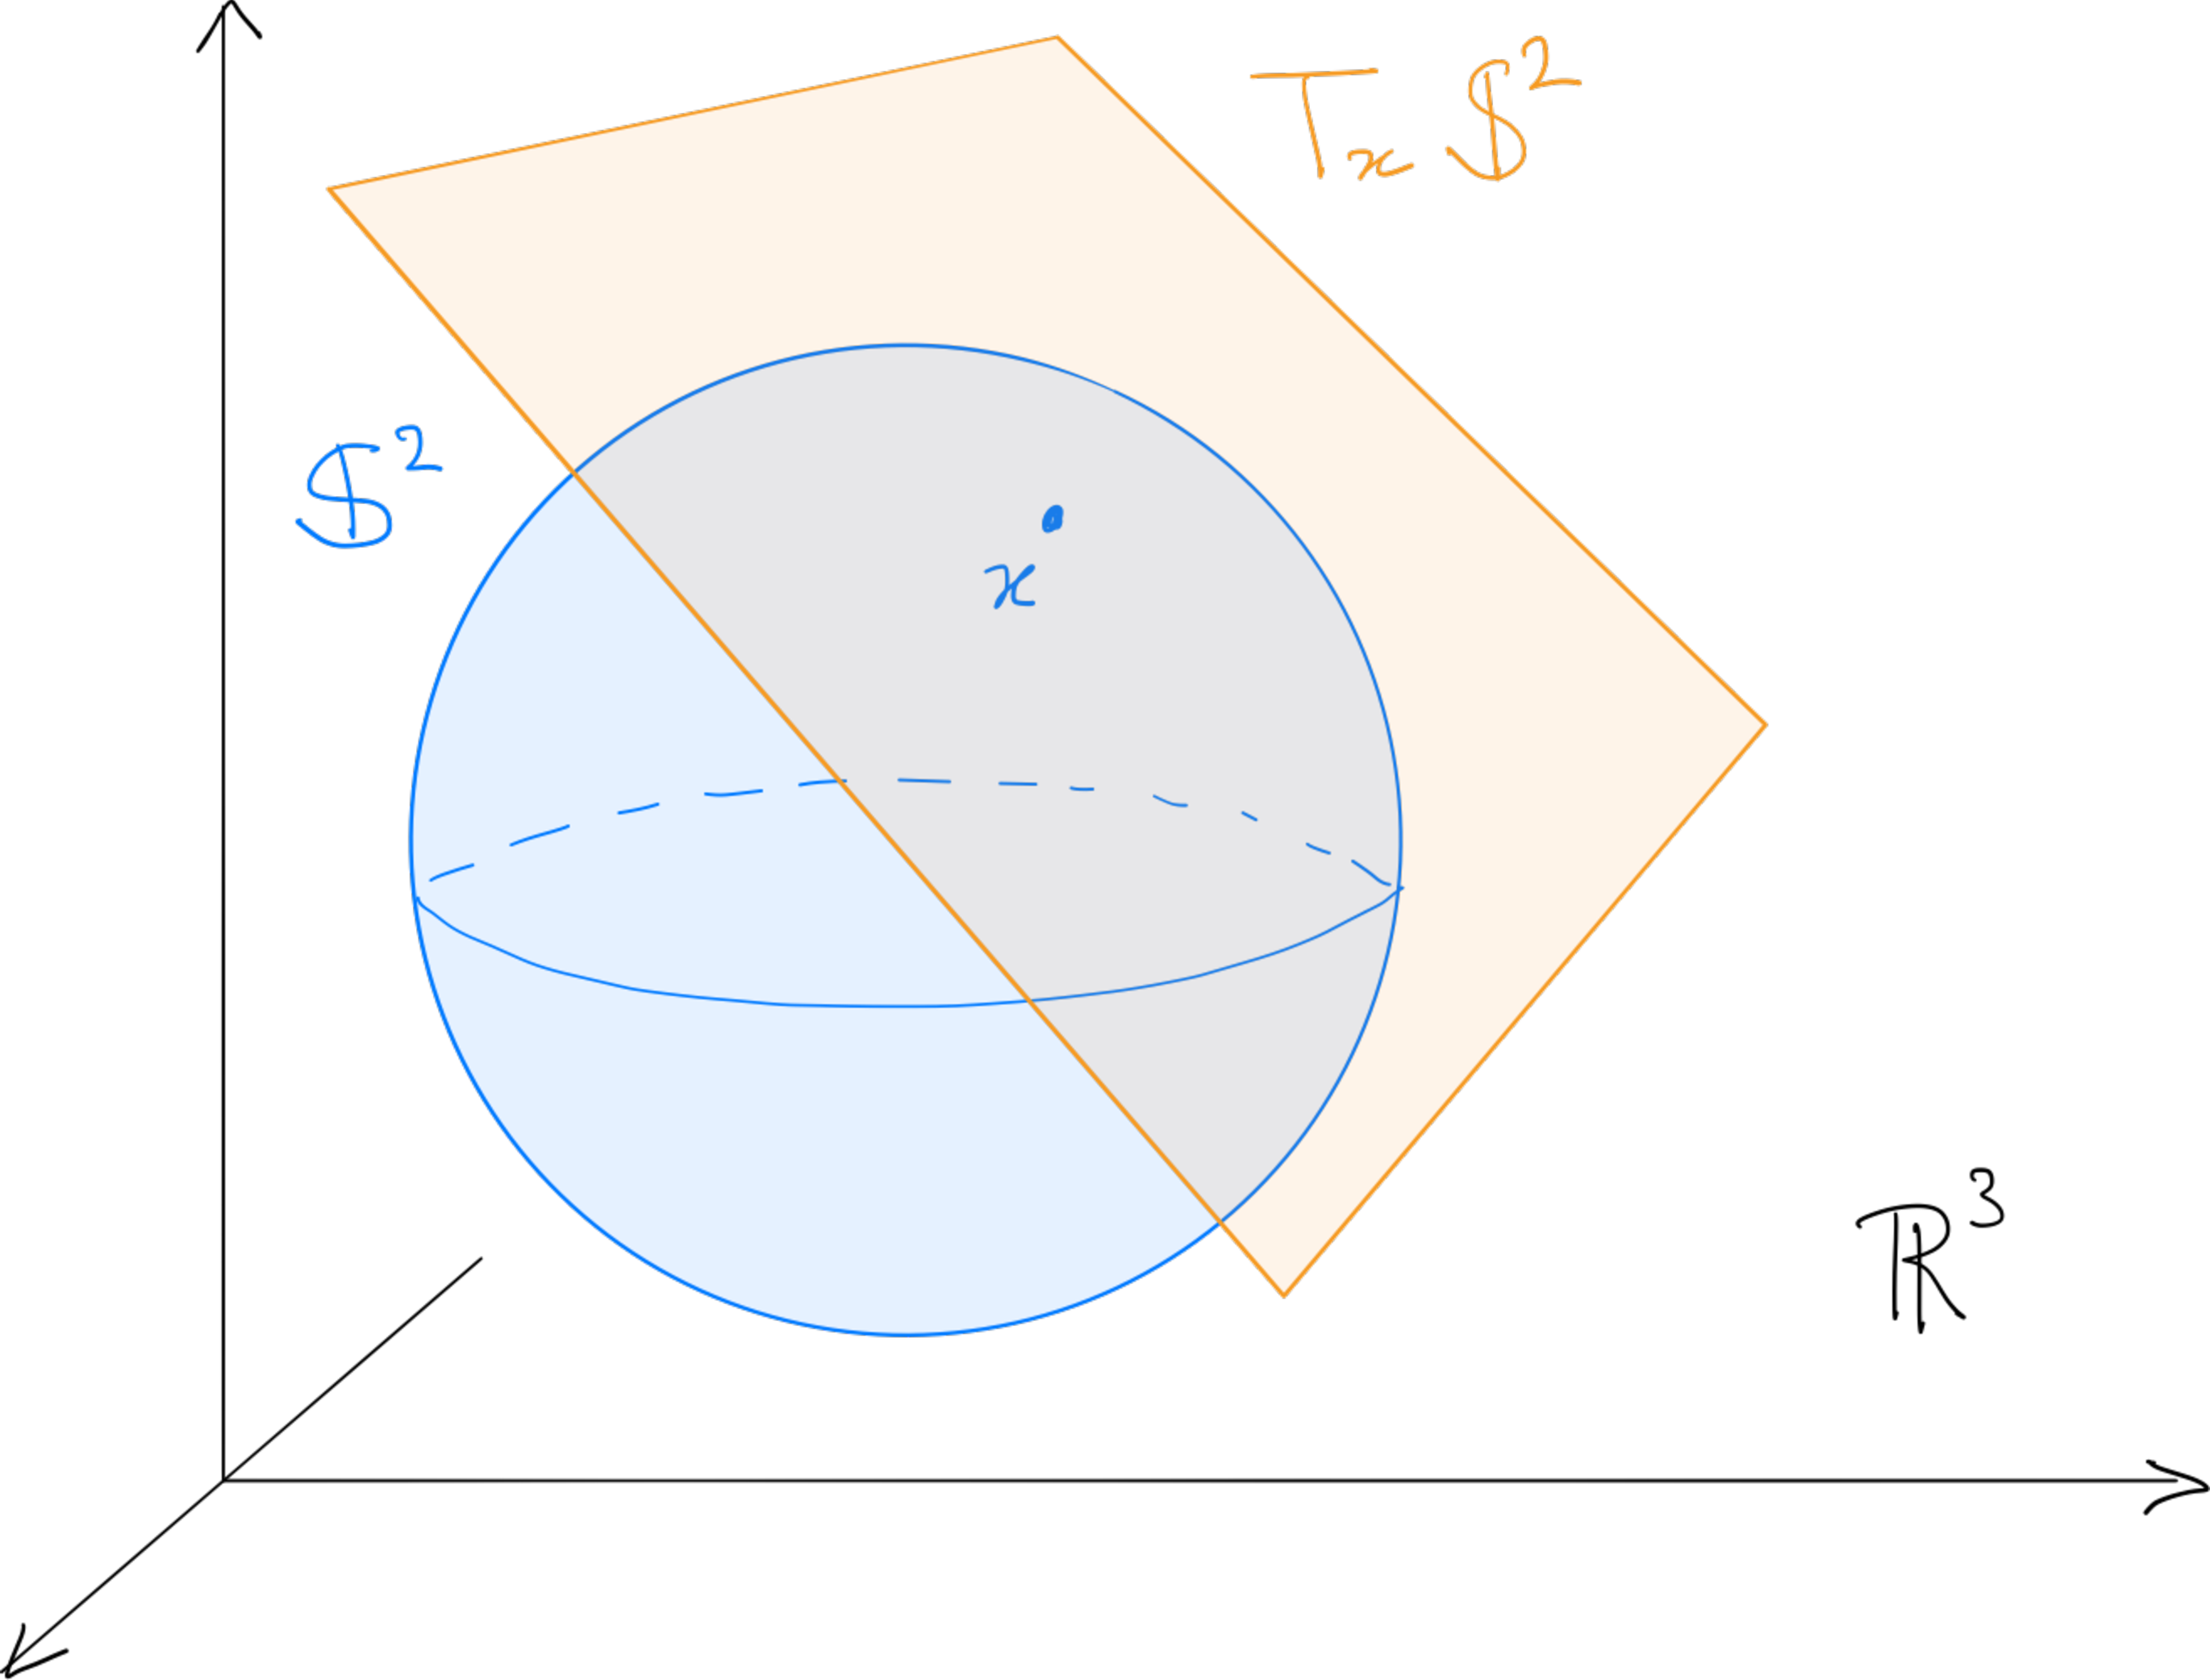
\includegraphics{2_1-embedded-sphere-tangent.pdf}
  \label{fig:tan-embedded-sphere}
  \caption{Tangent space to a point of a sphere $\bS^2$ embedded into the ambient space $\R^3$.}
\end{marginfigure}
In this chapter we will see how to associate to an $n$-dimensional smooth manifold $M$ an $n$-dimensional vector space, denoted by $T_x M$, to each point $x\in M$.
Such vector space is called \emph{tangent space to $M$ at $x$} and, for a manifold embedded into a euclidean ambient space, it will coincide with the intuitive understanding of a tangent hyperplane to the point on the manifold, see also Figure~\ref{fig:tan-embedded-sphere}.
As we will see, there are various different definition of tangent space but, in the end, they all turn out to be equivalent.

Due to the amount of freedom and the many equivalent definitions, there is no unique way of introducing tangent spaces.
Just to give you an idea, all the following approaches lead to equivalent definitions (see also \cite{book:lee}):
\begin{enumerate}
  \item equivalence classes of curves through a point;
  \item transformation laws of the components of vectors with respect to different charts;
  \item generalization of linear approximation into the idea of an abstract derivation;
  \item derivations in the category of germs of functions;
\end{enumerate}

It is also possible to ``flip'' the whole construction around, constructing differentials and cotangent spaces and using them to introduce the tangent spaces.
This is the approach taken by \cite{lectures:hitchin} and it is at least worth of a look if you want to see a different perspective.

To avoid diverging from the book too much, we will stick to derivations on the space of germs, which emphasizes the locality of derivations to an extreme.

The equivalence between such approach and the one based on speeds of curves and on derivations will be left as homeworks.

% \subsection{Partial derivatives}

% \newthought{Being locally euclidean seems to be very powerful}.
% Even though we are not yet in the position to define total derivatives of functions, we can already use the euclidean analogy in order to define partial derivatives.

% For simplicity, consider a smooth manifold $M$ of dimension $n$ and a function $f\in\cC^\infty(M,\R^n)$.

% Let $(U, \phi$) be a chart of $M$. 
% We already said that as a function on $\R^n$, $\phi$ has $n$ components $x^1, \ldots, x^n$ defined in terms of the standard euclidean coordinates $r^1, \ldots, r^n$ as $\phi^i = r^i \circ \phi$, $1\leq i\leq n$.
% For $p\in U$, the \emph{partial derivate $\frac{\partial f}{\partal x^i}$ of $f$ with respect to $x^i$ at $p$} can be defined as
% \begin{equation}
%   \frac{\partial}{\partial x^i}\big|_p f := 
%   \frac{\partial f}{\partial x^i} (p) :=
%   \frac{\partial f \circ \phi^{-1}}{\partial r^i} (\phi(p)) :=
% \end{equation}

\subsection{Directional derivatives}

Suppose that $f: U\subset\R^n\to\R^k$ is a smooth map defined on an open subset $U\subset \R^n$.
In multivariable calculus you have seen that if $x\in U$ and $v\in\R^n$, then the vector $Df(x) v$ can be interpreted as the directional derivative\footnote{Sometimes this is denoted $D_v f(x)$ instead.} of $f$:
\begin{equation}
    Df(x) v = \lim_{t\to0}\frac{f(x+tv) - f(x)}{t}.
\end{equation}
Then, the partial derivative is obtained as the particular case
\begin{equation}
    D_jf(x) := Df(x) e_j = \lim_{t\to0} \frac{f(x+te_j) - f(x)}{t}.
\end{equation}
Of course, we can also look at the derivative by using the standard euclidean coordinates $r^1, \ldots, r^n$, in that case we would be deriving $r^i \circ f : \R^n \to \R$.

Let's take it slow, and compare all these various derivatives next to each other.
For $f:U\subset\R^n\to\R^k$ and $x\in U$, we have
\begin{marginfigure}[3.5cm]
    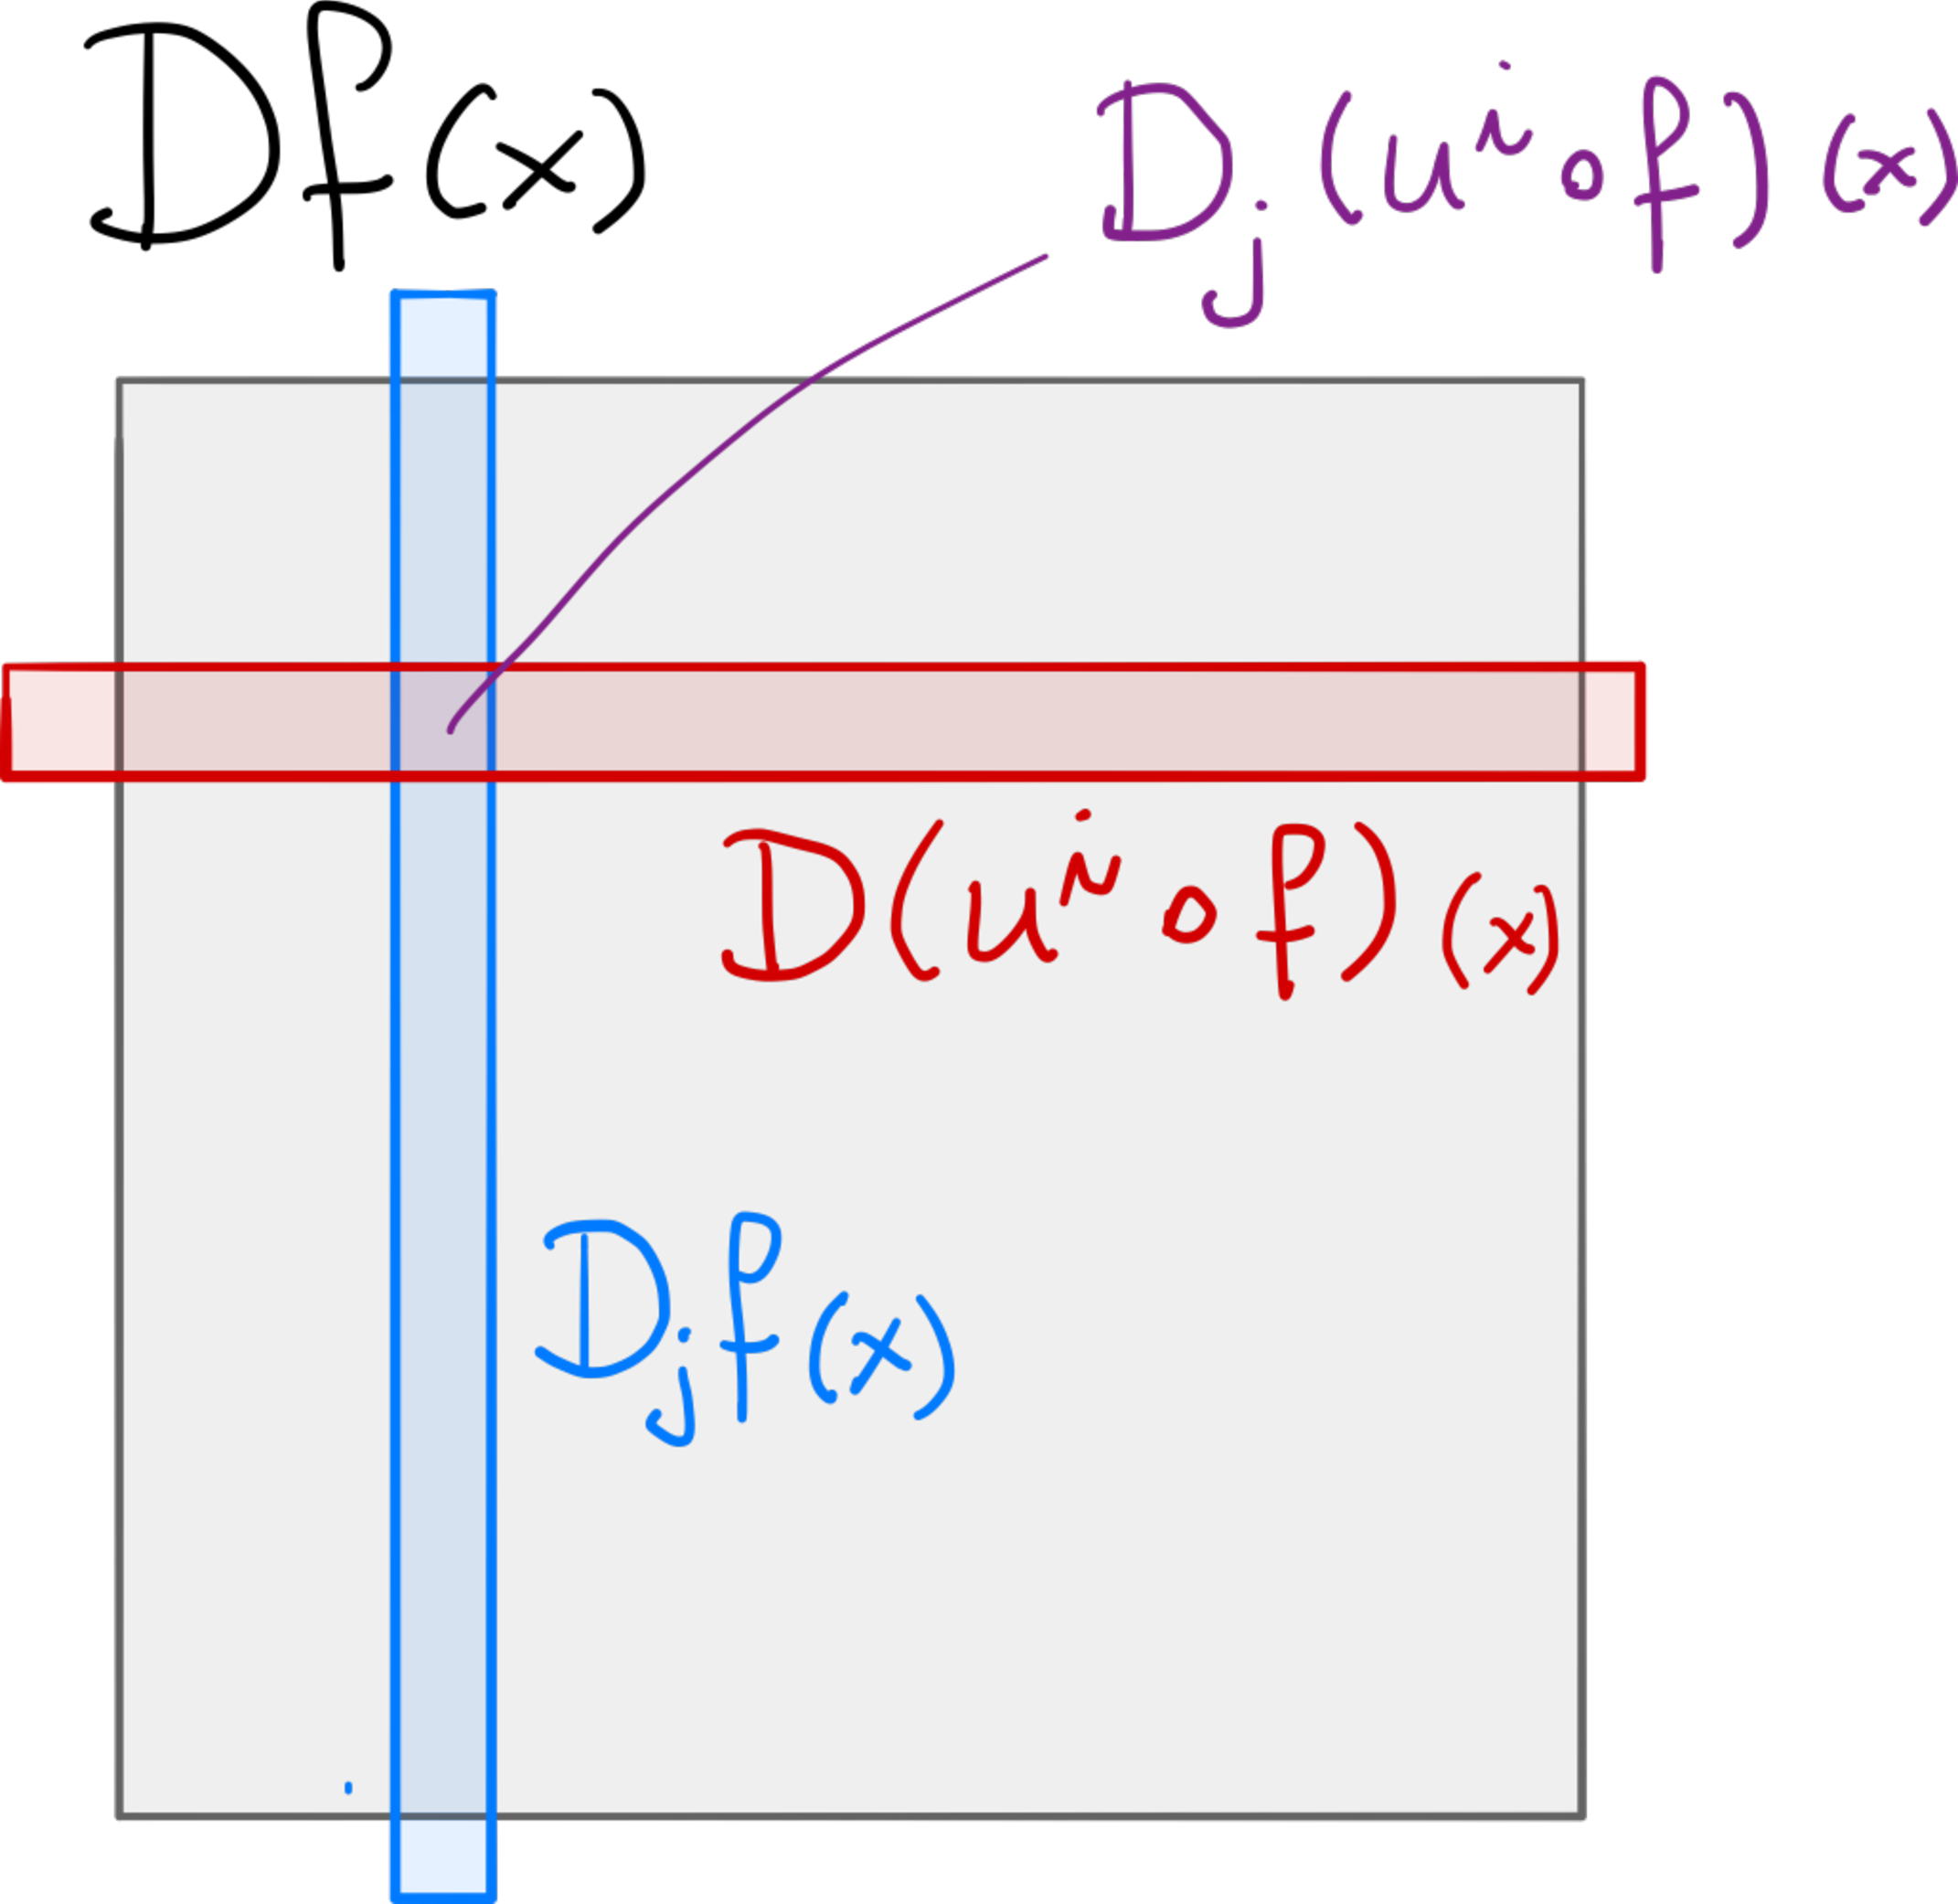
\includegraphics{2_3-ederivs.pdf}
\end{marginfigure}
\begin{itemize}
    \item $Df(x)$, the Jacobian matrix, which is a $k\times n$ matrix;
    \item $D_j f(x)$, the $j$th column of the matrix $Df(x)$, which is an element of $\R^k$;
    \item $D(r^i\circ f)(x)$, a linear function from $\R^n to \R$, which one can think as the $i$th row of the matrix $Df(x)$;
    \item $D_j(r^i\circ f)(x) = \frac{\partial f^i}{\partial x^j}(x)$, a number in $\R$, which corresponds to the element $(i,j)$ of the matrix $Df(x)$.
\end{itemize}

This notation using $D$ instead of spelling out the partial derivatives, comes with an important advantage.
Let's use it to rewrite the chain rule form Proposition~\ref{thm:chainrule}({thm:chainrule2}):
\begin{equation}
    D_j(u^i\circ g \circ f) (x) = \sum_{r=1}^k D_r(u^i\circ g)(f(x))\; D_j(u^r \circ f)(x),
    \qquad
    1\leq i\leq m, 1\leq j \leq n.
\end{equation}
As you cen see, we did not need to spell out explicitly the coordinate systems on $\R^n$ or $\R^k$.

\subsection{Speeds of curves}

A map $\gamma\in\cC^1(I, M)$ from an open interval $I\subset\R$ to a smooth manifold $M$ is called \emph{$\cC^1$-curve} on $M$.
\begin{marginfigure}
  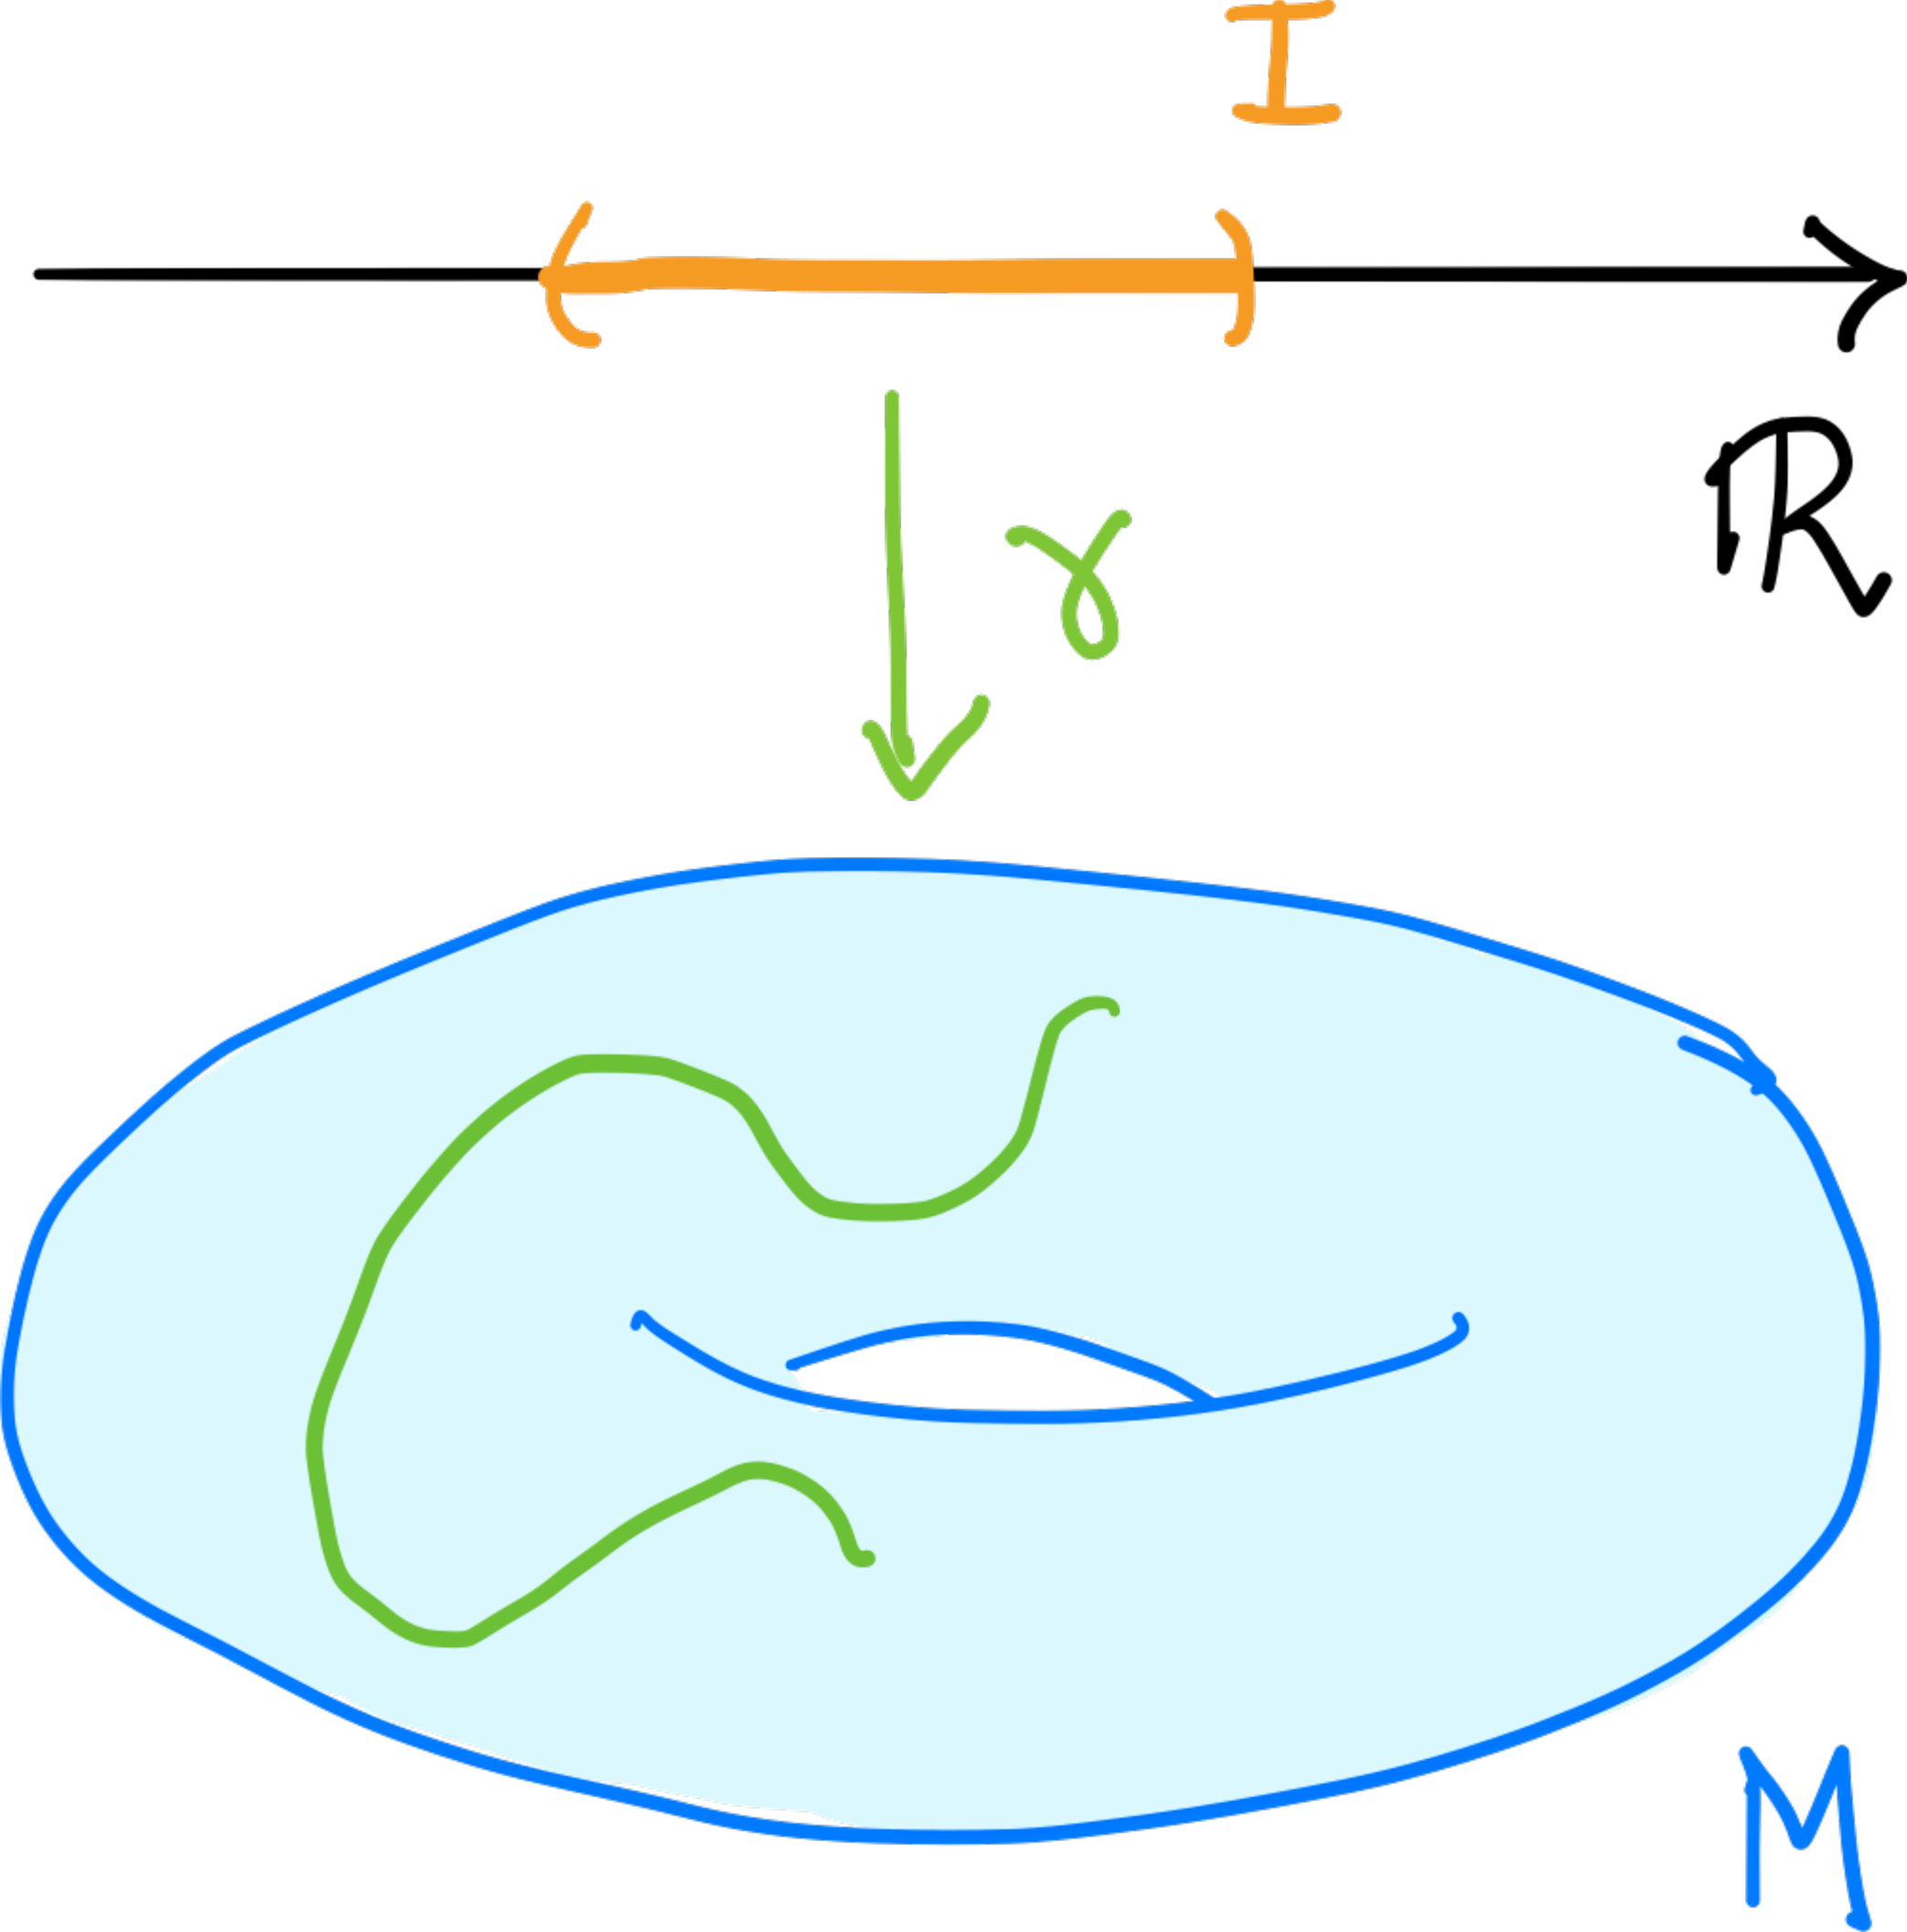
\includegraphics{2_2-curve-on-M.pdf}
\end{marginfigure}
F
\subsection{Via charts}
\subsection{As derivation}

\subsection{A summary}

\subsection{The tangent bundle}